The first part of this chapter is a summary of ~\cite[p. 4-7]{BuilAranda20131}. 
In the second part of this chapter we discuss the difference of the notions we
introduced in the first part.
In order to get a
deeper understanding of the SERVICE operator it is mandatory to understand which
problems occur when evaluating the SERVICE operator.
A direct implementation of the SERVICE operator based of the semantics is
infeasible in practice. Given $(\mbox{SERVICE }  x \
P_1)$, if $x$ is not restricted to a finite set, we would have to evaluate $P_1$ over every 
possible SPARQL endpoint in $dom(ep)$. This is obviously impossible. To ensure that $P_1$
only gets evaluated over a finite set of URIs, $x$ needs to be limited to exactly
those. In the W3C standard only indications are provided on how to evaluate the
service operator~\cite{w3standardservice} when the location is a variable and
not an URI. In~\cite{BuilAranda20131} the authors deal with this issue by
providing a notion of boundedness. In order to demonstrate how one could
evaluate a service operator using a variable to evaluate a query over more than
one endpoint the following example is given:
\begin{example}[\cite{BuilAranda20131}]
	Let $G$ be an RDF graph that uses triples of the form\\ $(a, service\_address,b)$
	with the intention to express that $b$ is a SPARQL endpoint URI with name $a$.
	Then we consider the following query $P$ over the graph $G$ in the dataset $DS$:
	\begin{align*}
		P=((x, service\_address, y) \AND (\mbox{SERVICE } y \ (z_n,email,z_e)))
	\end{align*}
	It is easy to see that $P$ is used to compute the list of names and email
	addresses that can be retrieved from the SPARQL endpoints stored in the RDF
	graph $G$ through the $service\_address$ triple. 
	The whole point of this example is to point out that there is a simple practical
	way to evaluate $P$ over $G$ that is also feasible:
	By evaluating $\ll (x,service\_address,y) \rr^{DS}_G$ first and then for every
	mapping $\mu$ in this set we further evaluate $\ll (\mbox{SERVICE } a \ (z_n, email, z_e)
	\rr^{DS}_G$, where $a = \mu(y)$. 
\end{example}
Throughout the chapter we will provide four different definitions on how the
destinations of a SERVICE-operator can be bounded within a graph pattern if the
destination is a variable. Those definitions were first introduced
in~\cite{BuilAranda20131}.
\begin{enumerate}
	\item Boundedness: Boundedness is a na{\"i}ve semantic approach to the
		problem. After formally defining the property, we will show that
		deciding whether a variable is bounded in a graph pattern
		is undecidable and thus not feasible for practical use.

	\item Strong boundedness: Strong boundedness is a syntactical approach to
		the problem. We will, by defining the property provide a recursive
		procedure on how to decide which variables in a graph pattern are
		strongly bounded. It will also be shown that if a variable is strongly
		bounded, it is bounded aswell. 
		Although this procedure would be feasible for practical
		use complexity-wise, it is not able to decide whether a graph pattern
		can be evaluated in practice. We will provide an example in form of a
		graph pattern which is feasible to be evaluated in practice but not
		strongly bounded.

	\item Service-boundedness: Service-boundedness would be the optimal solution for
		deciding which graph patterns can be evaluated in practice. If a pattern
		is service-bounded, it can be evaluated in practice. The problem however
		is, that the definition builds on the definition of boundedness which is
		undecidable. Therefore service-boundedness is not feasible for practical
		use.
	\item Service-safeness: The definition of service-safeness builds on the
		definition of strong boundedness. 
		service-safeness is easy to decide and we will show that if a pattern is
		service-safe, it is also service-bounded. This solution should be used in
		practice for the original problem.
\end{enumerate}

In the last section we will discuss the difference of boundedness and strong
boundedness (and thus service-boundedness and service-safeness because the
latter definitions build on former definitions). 

\section{The four different ways to bind the destination of a SERVICE-operator}

To describe boundedness we need three definitions namely the domain of a graph,
a dataset and a graph pattern.

\begin{definition}[Domain of a graph, a dataset and a graph pattern,\cite{BuilAranda20131}]
	The domain of a graph $G$ denoted $dom(G)$ is defined as $dom(G) = \bigcup\limits_{(u,v,w) \in G}
	vars(u,v,w)$. The domain of a dataset $DS$, denoted $dom(DS)$ is defined as
	$dom(DS) = \bigcup\limits_{G \in names(DS)} dom(G)$.
	The domain of a graph pattern $P$ is denoted $dom(P)$ and refers to the set of URIs that are
	mentioned in $P$.
\end{definition}

Boundedness of a variable $x$ in a graph pattern $P$ makes sure that the
variable is always in the domain of every solution $\mu$ and the image $\mu(x)$ is either in the 
domain of the dataset $P$ gets evaluated over, it is a graph name or it is in the domain of the pattern.

\begin{definition}[Boundedness,\cite{BuilAranda20131}]
	Let $P$ be a graph pattern and $x \in var(P)$. Then $x$ is bounded in $P$ if the
	following condition holds:
	For every dataset $DS$, every graph $G$ in $DS$ 
	and every $\mu \in \ll P \rr^{DS}_G:$\\
	\[ x \in dom(\mu) \mbox{ and } \mu(x) \in (dom(DS) \cup names(DS) \cup dom(P)). \]
\end{definition}

Resulting from this definition a very naive way to ensure that
a graph pattern $P$ can be evaluated in practice seems to arise:
Assuming we want to evaluate a subpattern $(\mbox{SERVICE } x \ P_1)$ of $P$
we require $x$ to be bounded in $P$. We can then define the problem for deciding if a variable
is bounded in a graph pattern $P$:

\begin{framed}\noindent \textbf{BOUND IN PATTERN}\\
	\textbf{INPUT:} A graph pattern $P$ and a variable $x \in var(P)$.\\
	\textbf{QUESTION:} Is $x$ bounded in $P$?
\end{framed}
Unfortunately \textbf{BOUND IN PATTERN} is undecidable which can be shown by
reducing from \textbf{SPARQL SAT} to \textbf{BOUND IN PATTERN}.
\begin{framed}\noindent \textbf{SPARQL SAT}\\
	\textbf{INPUT:} A graph pattern $P$.\\
	\textbf{QUESTION:} Does a dataset $DS$ and a graph $G$ in $DS$ exist such
	that $\ll P \rr^{DS}_G$?
\end{framed}
It is a well known result that $\textbf{SPARQL SAT}$ is undecidable~\cite{angles2008expressive}.

\begin{theorem}[\cite{BuilAranda20131}]\label{boundundec}
	\textbf{BOUND IN PATTERN} is undecidable.
\end{theorem}
\begin{proof}
	By providing a reduction from the \textbf{SPARQL SAT} problem to the
	\textbf{VARIABLE BOUND IN PATTERN} Problem we will be able to prove the theorem.
	Let $P$ be a graph pattern, i.e., an arbitrary instance of \textbf{SPARQL SAT} and
	$x,y,z$ variables not mentioned in $P$. Then define the graph pattern $Q$,
	i.e. the instance of \textbf{VARIABLE BOUND IN GRAPH} pattern as follows: $Q =
	((x,y,z) \UNION  P)$ and choose $x$ to be the potentially bounded variable.
	It remains to show that $x$ is bounded in $Q$  if and only if $P$ is not
	satisfiable.\\
	$(\Rightarrow)$:\\
	Assume now that the variable $x$ is bounded in $Q$, i.e., for every RDF graph $G$
	in $DS$ and every $\mu \in \ll Q \rr^{DS}_G:$ $x \in dom(\mu)$ and $\mu(x) \in
	(dom(DS) \cup names(DS) \cup dom(P))$. Let $DS$ be an arbitrary dataset and let
	$G$ be an arbitrary graph in $DS$. Distinguish the following two cases:
	\begin{enumerate}
		\item $\ll Q \rr^{DS}_G = \emptyset$. Because of $\ll Q \rr^{DS}_G =
			\emptyset$, we can instantly see that $P$ is unsatisfiable.
		\item $\ll Q \rr^{DS}_G \neq \emptyset$.\\
			Let $\mu \in \ll Q \rr^{DS}_G$ be arbitrary.
			We can instantly see that $x \in dom(\mu)$ must hold. 
			Because by construction $P$ doesn't contain $x$, 
			$\mu \notin \ll P \rr^{DS}_G$. Thus $P$ is unsatisfiable.
	\end{enumerate}
	\noindent$(\Leftarrow)$:\\
	Assume now that $P$ is not satisfiable. Let $DS$ be an arbitrary dataset and let
	$G$ be an arbitrary graph in $DS$. Because of our initial assumption $\ll P
	\rr^{DS}_G = \emptyset$. We will now further distinguish between two cases:
	\begin{enumerate}
		\item $\ll Q \rr^{DS}_G = \emptyset$. Then $x$ is trivially bounded in $Q$.

		\item $\ll Q \rr^{DS}_G \neq \emptyset$.\\
			Let $\mu \in \ll Q \rr^{DS}_G$ be arbitrary.
			We can instantly see by construction of $Q$ that $x \in
			dom(\mu)$ must hold. By SPARQL semantics $\mu(x) \in dom(DS)$. Thus $x$
			is bounded in $Q$.\qedhere
	\end{enumerate}
\end{proof} 

As deciding boundedness for a variable is undecidable the notion of
\emph{strong boundedness} is introduced, which is a syntactic condition and
efficiently verifiable. 

\begin{definition}[Strong
	Boundedness~\cite{BuilAranda20131}]\label{def:strongboundedness}
	Let $P$ be a graph pattern. Then the set of strongly bounded variables in $P$,
	denoted by $SB(P)$, is recursively defined as follows.

	\begin{itemize}
		\item if $P =t$, where $t$ is a triple pattern, then $SB(P) = vars(t)$;
		\item if $P = (P_1 \ AND \ P_2)$, then $SB(P) = SB(P_1) \cup SB(P_2)$ 
		\item if $P = (P_1  \ UNION \ P_2)$, then $SB(P) = SB(P_1) \cap SB(P_2)$ 
		\item if $P = (P_1 \ OPT \ P_2)$, then $SB(P) = SB(P_1)$ 
		\item if $P = (GRAPH \ u \ P_1)$, with $u \in U\cup V$, 
			then\\
			\begin{align*}
				SB(P) = 
				\begin{cases}
					SB(P_1) & \mbox{$u \in U$} \\
					SB(P_1) \cup \{u\} &\mbox{$u \in V$} 
				\end{cases}
			\end{align*}

		\item if $P = (SERVICE \ u \ P_1)$, with $u \in U \cup V$, then $SB(P) = \emptyset$.
	\end{itemize}
\end{definition}

It is a simple observation that this recursive definition collects a set of
variables that are guaranteed to be bounded in $P$. The following proposition
documents this observation.

\begin{proposition}[\cite{BuilAranda20131}]\label{sbinb}
	For every graph pattern $P$ and a variable $x \in var(P)$, if $x \in SB(P)$,
	then $x$ is bounded in $P$.
\end{proposition}
The proof is a very straight forward induction and can be found
in~\cite[Appendix A]{BuilAranda20131}.

We notice that this proposition is not an if and only if statement and hence we may be
able to provide a pattern $P$ where variables $x \in vars(P)$ exist, which are
bounded but not
strongly bounded. Furthermore another example is provided which makes things more
complicated. In Example~\ref{ex:boundedbad} we provide a graph pattern $P$ where a variable in the
destination of a SERVICE-operator occurs which is neither bounded nor strongly
bounded. We will then provide a plan on how to evaluate $P$ and thus show that
the definition of neither boundedness nor strongly boundedness is sufficient for
practical usage. 

\begin{example}\label{ex:boundedbad}
	Consider the following graph pattern:
	\begin{align*}
		P_1 = [(x,service\_description,z) \UNION ((x,service\_address, y) \AND
			\\\
		(\mbox{SERVICE } y \ (x_n,email,x_e)))]
	\end{align*}
	The variables $x$ and $z$ store the name of a SPARQL endpoint and a description of its
	functionalities through the $service\_description$ triple. The variables $x$ and $y$ store the
	name of a SPARQL endpoint and the URI where it is located through the
	service\_address triple. The problem is, that variable $y$ is neither
	bounded nor
	strongly bounded in $P_1$. However we can still easily evaluate the pattern by
	assuming a dataset $DS$ and an RDF graph $G$ in $DS$:\\
	Compute $\ll (x, service\_description,z)\rr^{DS}_G$, then compute \\
	$\ll (x, service\_addres,y) \rr^{DS}_G$ and finally for every
	$\mu \in \ll (x, service\_addres,y) \rr^{DS}_G$, compute $\ll (\mbox{SERVICE }
	a \ (x_n,email,x_e))\rr^{DS}_G$ with $a = \mu(y)$. We can easily see that $y$ is
	bounded and strongly bounded in the subpattern \\ $((x,service\_address, y) \AND
	(\mbox{SERVICE } y \ (x_n,email,x_e)))$ of $P_1$ and thus the evaluation is possible.
\end{example}

\noindent To describe a condition that ensures all SPARQL queries containing the SERVICE
operator can be evaluated in practice, the definition of Service-Boundedness is
introduced. The definition of service-boundedness uses a parse tree to make sure
that our evaluation takes bounded subpatterns into account.

\begin{example}\label{ex:parsetree}[\cite{BuilAranda20131}]
	Parse tree $\T(Q)$ for the graph pattern \\ $Q = ((y,a,z) \UNION ((x,b,c) \AND (\mbox{SERVICE } x \ (y,a,z))))$.

	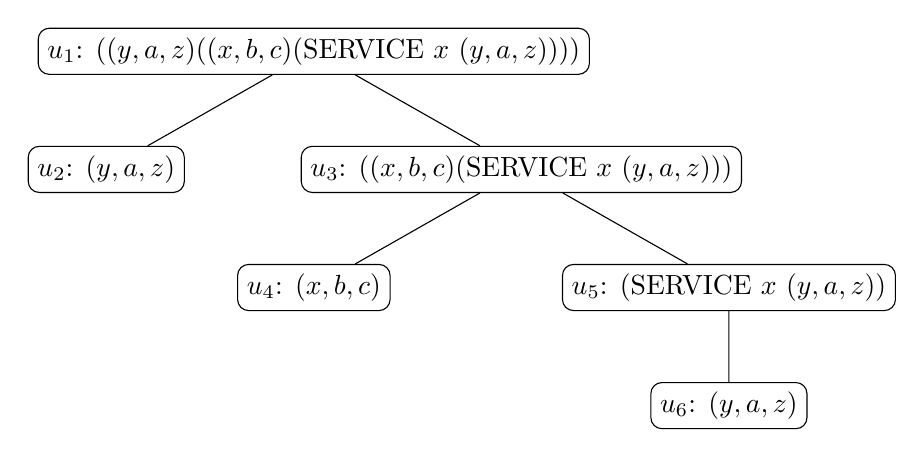
\begin{tikzpicture}[sibling distance=15em,
			every node/.style = {shape=rectangle, rounded corners,
	draw, align=center, top color=white}]]
	\node {$u_1$: $((y,a,z) \UNION ((x,b,c) \AND (\mbox{SERVICE } x \ (y,a,z))))$}
	child { node {$u_2$: $(y,a,z)$} }
	child { node {$u_3$: $((x,b,c) \AND (\mbox{SERVICE } x \ (y,a,z)))$}
		child { node {$u_4$: $(x,b,c)$}}
		child { node {$u_5$: $(\mbox{SERVICE } x \ (y,a,z))$}
	child	{ node {$u_6$: $(y,a,z)$}} }};
\end{tikzpicture}

\end{example}

\begin{definition}[Parse Tree, \cite{BuilAranda20131}]
	A parse tree of a graph pattern $P$, $\T(P)$ is a tree where each
	node is a sub-pattern of $P$. Each node has an identifier.
	In the parse tree the child relation is used to store the structure of the
	sub-patterns of the graph pattern. The root of the parse tree contains the pattern $P$. Then, 
	in the child(ren) of $P$ the pattern is split up into the respective sub-pattern(s). This is done recursively 	until a node contains only a triple. 
	%Assume we have a SPARQL pattern $P$. 
	%	We will construct the parse tree $(V,E,r,\lambda)$, where $V$ is the set of vertices, 
	%	$E$ the set of edges, $r$ the root and $\lambda$ a labelling function as follows:


\end{definition}
In Example~\ref{ex:parsetree} a parse tree can be found

Using the definition of a Parse Tree, Service-Boundedness can be defined.

\begin{definition}[\cite{BuilAranda20131}]
	A graph pattern $P$ is service-bounded if for every node $u$ of $\T(P)$ with
	label $(SERVICE \ x\  P_1)$, it holds that
	\begin{enumerate}
		\item there exists a node $v$ of $\T(P)$ with label $P_2$ such that $v$
			is an ancestor of $u$ in $\T(P)$ and $x$ is bounded in $P_2$,
		\item $P_1$ is service-bounded.
	\end{enumerate}
\end{definition}

Corresponding to this definition we will introduce the \textbf{SERVICE BOUND}
problem:
\begin{framed}\noindent \textbf{SERVICE BOUND}\\
	\textbf{INPUT:} A graph pattern $P$.\\
	\textbf{QUESTION:} Is $P$ service-bounded?
\end{framed}

Intuitively one can already imagine that deciding the \textbf{SERVICE BOUND}
problem is undecidable because it uses boundedness in it.

\begin{theorem}[\cite{BuilAranda20131}]
	\textbf{SERVICE BOUND} is undecidable.
\end{theorem}
\begin{proof}
	By providing a reduction from the \textbf{SPARQL SAT} problem to the  
	\textbf{SERVICE BOUND} problem we will be able to show undecidability.
	Let $P$ be a graph pattern, i.e., an arbitrary instance of \textbf{SPARQL SAT} and
	$x,y,z,x',y',z'$ variables not mentioned in $P$.
	Also assume that $P$ does not mention the operator SERVICE which is not required
	to make the SPARQL satisfiability problem undecidable.
	Then define the graph pattern $Q$, i.e., the instance of \textbf{SERVICE BOUND} as: 
	\begin{align*}
		Q = (((x,y,z) \UNION  P) \AND (\mbox{SERVICE } x \ (x', y', z'))).
	\end{align*}

	\noindent It remains to show that $Q$ is service-bounded if and only if $P$ is not
	satisfiable.

	\bigskip\noindent
	$(\Leftarrow)$ \quad If $P$ is not satisfiable, then $Q$ is equivalent to the
	pattern: 
	\begin{align*}
		Q' = ((x,y,z)) \AND (\mbox{SERVICE} \ x \ (x', y', z')).
	\end{align*} 
	But $Q'$ is service bounded because $x$ is bounded in $Q'$: Assume an
	arbitrary dataset $DS$, let $G$ be in $DS$. Then 
	for any $\mu \in \ll Q' \rr^{DS}_G$, $x \in dom(\mu)$ and for sure $\mu(x) \in
	(dom(DS) \cup names(DS) \cup dom(P))$ by semantics of SPARQL and the fact that
	$x$ occurs in the triple pattern $(x,y,z)$.


	\bigskip\noindent
	$(\Rightarrow)$\quad Assume that $P$ is satisfiable. Then we know that variable
	$x \not\in vars(P)$ and thus we have that $x$ is not a bounded variable in $Q$,
	and thus because $x$ occurs in a service operator, $Q$ is not service
	bounded.
\end{proof}

As the problem of undecidability prevails with the definition of
service-boundedness, we can again use the syntactic condition, i.e., strong boundedness to define
service-safeness which is the same as service-boundedness but uses strong
boundedness instead of boundedness. We know from
Definition~\ref{def:strongboundedness} that evaluating if a variable is strongly
bounded in a graph pattern can be done efficiently.

\begin{definition}[Service Safeness~\cite{BuilAranda20131}]
	A graph pattern $P$ is service-safe if for every node $u$ of $\T(P)$ with
	label $(SERVICE \ x \ P_1)$ it holds that:
	\begin{enumerate}
		\item there exists a node $v$ of $\T(P)$ with label $P_2$ such that $v$
			is an ancestor of $u$ in $\T(P)$ and $x \in SB(P_2)$.
		\item $P_1$ is service safe.
	\end{enumerate}
\end{definition}

As corollary to Proposition 1, the following proposition is obtained:
\begin{proposition}[\cite{BuilAranda20131}]
	If a graph pattern $P$ is service-safe, then $P$ is service-bounded.
\end{proposition}

\section{Boundedness and strong boundedness}
An interesting question is stirred up through introducing the notions of
boundedness and strong boundedness: What is the difference between the two
notions? 
Because boundedness is not equivalent to strong boundedness, there
must be patterns which are bounded but not strongly bounded. The following problem could arise:
Assume a pattern is bounded but not strongly bounded. Then it is feasible to be evaluated, 
but the proposed algorithm returns that it is not.

\begin{example}\label{bbutnotsbound}
	\begin{align*}
		P = ((x,a, b) \OPT (x, a, y)).
	\end{align*}
	We can see that $y$ is bounded in $P$ because for every RDF graph $G$ in $DS$ and
	every $\mu \in \ll P \rr^{DS}_G$ we have that $y \in dom(\mu)$ and
	$\mu(y) \in (dom(DS))$: Assume we have a $\mu \in \ll P \rr^{DS}_G$. Then $x
	\in dom(\mu)$ by semantics of OPT. Assume w.l.o.g. $\mu(x) = c$. Then
	$(c,a, b) \in G$. But then the mapping $\{ x \mapsto c , y\mapsto b \}
	\in \ll P \rr^{DS}_G$.
	The set of strongly bounded variables, i.e., $SB(P) = \{ x \}$ by
	Definition~\ref{def:strongboundedness} contains only $x$.
\end{example}
Example~\ref{bbutnotsbound} shows that there are patterns which are bounded but not strongly bounded. 
One could easily resolve the problem of Example~\ref{bbutnotsbound} and make $y$
strongly bounded again: 
It is easy to see that $((x,a, b) \OPT (x, a, y)) \equiv ((x,a, b) \AND (x, a,
y))$ holds. Thus we replace the graph pattern $P$ with the graph pattern $Q = ((x,a, b) \AND (x, a, y))$. 
While preserving the meaning of $P$, $Q$ also makes sure that $y$ is now strongly bound
in $Q$, i.e., $SB(Q) = \{ x, y\}$. 

Example~\ref{bbutnotsbound} also elicits a new question: Could deciding boundedness be
feasible in fragments of SPARQL where the problem \textbf{EQUIVALENCE} is
decidable? An idea for a decision procedure of \textbf{BOUND IN PATTERN} is illustrated
in Algorithm~\ref{bsbalgorithm}. This procedure would not contradict the results
of Theorem~\ref{boundundec} because in Theorem~\ref{boundundec} general SPARQL
is considered and it is a well known result that \textbf{EQUIVALENCE} is
undecidable in general SPARQL.

\begin{algorithm}
	\caption{BSB}\label{bsbalgorithm}
	INPUT: pattern $P$ and $x \in \mathit{vars}(P)$\\
	If $x \in SB(P)$ return true;\\
	For all subpatterns $(P_1 \OPT P_2)$ of $P$:\\
	If $(P_1 \OPT P_2) \equiv (P_1 \AND P_2)$ holds, replace $(P_1 \OPT
	P_2)$ with $(P_1 \AND P_2)$ in $P$.\\
	Call the resulting graph pattern
	$Q$.\\
	If $(x \in \mathit{SB}(Q))$ return true;\\
	else return false;
\end{algorithm}

%\begin{framed}\noindent \textbf{EQUIVOPT}\\
%	\textbf{INPUT:} A graph pattern $P$ and a variable $x \in \mathit{vars}(P)$
%	which is not strongly bound in $P$.\\
%	\textbf{QUESTION:} Is there a graph pattern $Q$, where $P \equiv Q$ 
%	and $Q$ replaced all subpatterns $(P_1 \OPT P_2)$ of $P$
%	with $(P_1 \AND P_2)$ in $Q$ where $(P_1 \OPT P_2) \equiv (P_1 \AND P_2)$ holds? 
%\end{framed}

%\begin{theorem}\label{ezprop}
%	Let $P$ be a graph pattern in a SPARQL fragment $\mathbf{P}$ and $x \in
%	\mathit{vars}(P)$. The problem of deciding whether $x$ is bounded in $P$ can
%	be reduced to the problem whether $((P_1 \OPT P_2) \equiv (P_1 \AND P_2))$
%	for all subpatterns $(P_1 \OPT P_2)$ of $P$. 
%\end{theorem}
%\begin{proof}
%	Consider the following decision procedure:
%	\begin{algorithm}
%		\caption{BSB}
%		INPUT: pattern $P$ and $x \in \mathit{vars}(P)$\\
%		If $x \in SB(P)$ return true;\\
%		For all subpatterns $(P_1 \OPT P_2)$ of $P$:\\
%		If $(P_1 \OPT P_2) \equiv (P_1 \AND P_2)$ holds, replace $(P_1 \OPT
%		P_2)$ with $(P_1 \AND P_2)$ in $P$.\\
%		Call the resulting graph pattern
%		$Q$.\\
%		If $(x \in \mathit{SB}(Q))$ return true;\\
%		else return false;
%	\end{algorithm}
%\end{proof}
%
%Notice that the decision procedure $BSB$ uses a subprocedure to decide $(P_1
%\OPT P_2) \equiv (P_1 \AND P_2)$.
%Let $(P,x)$ be an arbitrary instance of \textbf{BOUNDED IN PATTERN}.
%It remains to show that $\textit{BSB}(P,x)$ returns true iff $x$ is bounded in
%$P$. 
%If $BSB$ returns true from 1. We know from Proposition~\ref{sbinb} that $x$ is
%bounded in $P$ and we are done.
%
%Assume now that $\textit{BSB}(P,x)$ returned true from line 6.
%By construction of BSB and the fact that $x \notin SB(P)$ we know that there was
%a subpattern $(P_1 \OPT P_2)$ in $Q$ where $(P_1 \OPT P_2) \equiv (P_1 \AND
%P_2)$ was true and $x \in \vars(P_2)$. It remains to show that $x$ is bounded in
%$P$.
%Let $\mathit{DS}$ be an arbitrary dataset and $G$ a graph in $\mathit{DS}$.
%Case distinction:
%\begin{enumerate}
%	\item $\ll P \rr^{\DS}_{G}$ is empty: then $x$ is trivially bounded in $P$.
%	\item Let $\mu \in \ll P \rr^{\DS}_G$:
%		We can use the fact that $x \in SB(Q)$ and $x \notin SB(P)$. Thus there
%		must have been at least one subpattern $(P_1 \OPT P_2)$ where $(P_1 \OPT
%		P_2) \equiv (P_1 \AND P_2)$ was true. By the fact that $x \in SB(Q)$ and
%		Proposition~\ref{sbinb} we know that $x$ is bounded in $Q$.
%		Because we only substitute the subpatterns of $P$ with equivalent
%		subpatterns,i.e. $(P_1 \OPT P_2)$ with $(P_1 \AND P_2)$, to receive $Q$
%		we know that $Q \equiv P$. Thus $x \in dom(\mu)$ and $\mu(x) \in
%		(dom(DS) \cup names(DS) \cup dom(P))$ holds and thus $x$ is bounded in
%		$P$.
%\end{enumerate}
%Assume that $x \notin SB(Q)$(line 7).
%We need to prove that $x$ is not bounded in $P$ and because again $Q \equiv
%P$, it suffices to show that $x$ is not bounded in $Q$. \\
%%Proof by contradiction:\\
%%Assume $x$ was bounded in $Q$. By assumption we know that for every dataset
%%$DS$, every graph $G$ in $DS$ and every $\mu \in \ll Q\rr^{DS}_G$:
%%$x \in dom(\mu)$ and $\mu(x) \in(dom(DS) \cup names(DS) \cup dom(Q))$.
%%Because $x \notin SB(Q)$ we know that there must have been a subpattern in $Q$,
%%call it $Q'$, where $x \in vars (Q')$, but $x \notin SB(Q')$ because $x \in
%%\vars(Q)$. 
%We also know that there are no subpatterns $(P_1 \OPT P_2)$ in $Q$
%where $(P_1 \OPT P_2) \equiv (P_1 \AND P_2)$ holds.
%We will show the following statement by induction on the structure of $Q$: 
%If $x \notin SB(Q)$ then $x$ is not bounded in $Q$. Obviously $x$ is not
%bounded in $Q$ if it holds because we assumed $x \notin SB(Q)$ and $x \in
%\vars(Q)$.
%\begin{itemize}
%	\item BC: $Q = t$, we have a case distinction: 
%		\begin{enumerate}
%			\item If $x \in \vars(t)$ the implication holds as $SB(Q) = \vars(t)$ and
%
%			\item$x \notin vars(t)$:
%				If $x \notin vars(t)$ the implication holds:
%				Let $\DS$ be a dataset and $G$ be a graph in $DS$ where $\ll t
%				\rr^{\DS}_G \neq \emptyset$ holds. Let $\mu \in \ll t
%				\rr^{\DS}_G \neq \emptyset$. By SPARQL semantics $x \notin dom(\mu)$.
%		\end{enumerate}
%
%	\item IS: $Q = (Q_1 \AND Q_2)$. 
%		Again case distinction:	
%		\begin{enumerate}
%			\item If $x \in vars(Q)$:
%				By definition of $SB$, we have that $SB(Q) = SB(Q_1) \cup SB(Q_2)$.
%				By induction hypothesis we have that if $x \notin SB(Q_i)$,
%				$i = 1,2$ then $x$ is not bounded in $Q_i$.
%				Assume now that $x \notin SB(Q)$. We know by
%				semantics of $SB$ that thus $x \notin SB(Q_i)$ for $i=1,2$.
%				Thus $x$ is not bounded in $Q_i$ for $i=1,2$. Thus there must
%				have been datasets $DS_i$ and a graphs $G_i$ such that 
%				there is a $\mu_i \in \ll Q_i \rr^{DS_i}_{G_i}$:
%				where either $x \notin dom(\mu_i)$ or $\mu_i(x) \notin (dom(DS_i) \cup
%				names(DS_i) \cup dom(Q_i))$, $i=1,2$.
%				Case distinction:
%				\begin{enumerate} 
%					\item If $x \notin dom(\mu_i)$ for $i=1,2$.	
%
%				\end{enumerate}
%			\item $x \notin vars(Q)$: 
%				Let $\DS$ be a dataset and $G$ be a graph in $DS$ where $\ll Q
%				\rr^{\DS}_G \neq \emptyset$ holds. Let $\mu \in \ll Q
%				\rr^{\DS}_G \neq \emptyset$. By SPARQL semantics $x \notin dom(\mu)$.
%		\end{enumerate}
%	\item IS: $Q = (Q_1 \UNION Q_2)$.
%		Again case distinction:	
%		\begin{enumerate}
%			\item If $x \in vars(Q)$:
%				By definition of $SB$, we have that $SB(Q) = SB(Q_1) \cap SB(Q_2)$.
%				By induction hypothesis we have that if $x \notin SB(Q_i)$,
%				$i = 1,2$ then $x$ is not bounded in $Q_i$.
%				Assume now that $x \notin SB(Q)$. We know by
%				semantics of $SB$ that thus $x \notin SB(Q_i)$ for $i=1$ or $i=2$ or both.
%				Thus $x$ is not bounded in $Q_i$ for $i=1$, $i=2$ or both. Thus there must
%				have been datasets $DS_i$ and a graphs $G_i$ such that 
%				there is a $\mu_i \in \ll Q_i \rr^{DS_i}_{G_i}$:
%				where either $x \notin dom(\mu_i)$ or $\mu_i(x) \notin (dom(DS_i) \cup
%				names(DS_i) \cup dom(Q_i))$, $i=1$ or $i=2$ or both.
%				W.l.o.g. assume $x$ is not bounded in $Q_1$. Then take
%				the counterexample,i.e. $DS_1$ and $G_1$ and consider $\ll Q
%				\rr^{DS_1}_{G_1}$. Because $x$ was not bounded in $\ll Q_1
%				\rr^{DS_1}_{G_1}$ we had a mapping $\mu_1$ where the definition
%				of boundedness was not fulfilled. By semantics of
%				$\mbox{UNION}$ we have that $\mu_1 \in \ll Q \rr^{DS_1}_{G_1}$. Thus $x$ is
%				not bounded in $Q$.
%			\item $x \notin vars(Q)$: 
%				Let $\DS$ be a dataset and $G$ be a graph in $DS$ where $\ll Q
%				\rr^{\DS}_G \neq \emptyset$ holds. Let $\mu \in \ll Q
%				\rr^{\DS}_G \neq \emptyset$. By SPARQL semantics $x \notin dom(\mu)$.
%		\end{enumerate}
%	\item IS: $Q = (Q_1 \OPT Q_2)$.
%		Again case distinction:	
%		\begin{enumerate}
%			\item If $x \in vars(Q)$:
%				By definition of $SB$, we have that $SB(Q) = SB(Q_1)$.
%				By induction hypothesis we have that if $x \notin SB(Q_i)$,
%				$i = 1,2$ then $x$ is not bounded in $Q_i$.
%				Assume now that $x \notin SB(Q)$. We know by
%				semantics of $SB$ that thus $x \notin SB(Q_1)$.
%				Thus $x$ is not bounded in $Q_1$. Thus there must
%				have been a dataset $DS_1$ and a graph $G_1$ such that 
%				there is a $\mu_1 \in \ll Q_1 \rr^{DS_1}_{G_1}$:
%				where either $x \notin dom(\mu_1)$ or $\mu_1(x) \notin (dom(DS_1) \cup
%				names(DS_1) \cup dom(Q_1))$.
%				Take the counterexample, i.e. $DS_1$ and $G_1$ and consider $\ll Q
%				\rr^{DS_1}_{G_1}$. Because $x$ was not bounded in $\ll Q_1
%				\rr^{DS_1}_{G_1}$ we had a mapping $\mu_1$ where the definition
%				of boundedness was not fulfilled. 
%				Case distinction:
%				\begin{enumerate}
%					\item If $\mu_1(x) \notin (dom(DS_1) \cup names(DS_1) \cup dom(Q_1))$
%						caused the problem then by semantics of
%						$\mbox{OPT}$ we have that $\mu_1 \cup A \in \ll Q
%						\rr^{DS_1}_{G_1}$. $A$ cannot change the value $\mu_1(x)$ had. Thus $x$ is
%						not bounded in $Q$.
%					\item If $x \notin dom(\mu_1)$
%							
%				\end{enumerate}
%			\item $x \notin vars(Q)$: 
%				Let $\DS$ be a dataset and $G$ be a graph in $DS$ where $\ll Q
%				\rr^{\DS}_G \neq \emptyset$ holds. Let $\mu \in \ll Q
%				\rr^{\DS}_G \neq \emptyset$. By SPARQL semantics $x \notin dom(\mu)$.
%		\end{enumerate}
%\end{itemize}


%\begin{theorem}\label{ezprop}
%	The problem of verifying, given a graph pattern $P$ in a SPARQL fragment
%	$\mathbf{P}$ and a variable $x \in
%	var(P)$, whether $x$ is bounded in $P$ is as hard as deciding $(P_1 \AND 
%	P_2)
%	\equiv (P_1 \OPT P_2)$ %for every subpattern $(P_1 \OPT  P_2)$ of $P$% 
%	in the SPARQL fragment $\mathbf{P}$.
%\end{theorem}
%\begin{proof}
%	It is very easy to decide strong boundedness and Proposition~\ref{sbinb}
%	shows that if a variable $x$ is in $SB(P)$ then $x$ is also bounded in $P$.
%	We thus modify our pattern $P$ in such a way, that $SB(P)$ collects all the
%	variables which are bounded, even those which are only bounded but not strongly
%	bounded.
%	Assume $x$ is bounded in $P$ and $x \notin SB(P)$.
%	There must thus be a subpattern $Q$ where $x \in vars(Q)$ but $x \notin
%	SB(Q)$. We will go through every step of the recursive approach of
%	Definition~\ref{def:strongboundedness} to find the subpattern where $x \in
%	vars(Q)$, $x \notin	SB(Q)$ but $x$ is bounded in $Q$.
%	\begin{itemize}
%		\item If $Q$ is a triple $t$ then $SB(Q) = var(t)$ and by assumption
%			that $x \in vars(Q)$ we get that $x \in SB(Q)$. 
%
%		\item If $Q$ is $(P_1 \AND P_2)$ then $SB(Q) = SB(P_1) \cup SB(P_2)$. By
%			assumption we know that $x \in vars(Q)$. By semantics of $\cup$ we
%			get that $x \in SB(Q)$. 
%			
%		\item If Q is $(P_1 \UNION  P_2)$ then $SB(P) = SB(P_1) \cap SB(P_2)$.
%			By assumption we have that $x \in vars(P_1 \UNION P_2)$.
%			Assume $x \notin SB(Q)$. 
%			We have a case distinction:
%			\begin{enumerate}
%				\item $x \in SB(P_1)$ and $x \in SB(P_2)$.
%				 We instantly see by semantics of $\cap$ that $x \in SB(Q)$. 
%
%				\item Assume w.l.o.g. that $x \in SB(P_1)$ but $x \notin SB(P_2)$. 
%					This contradicts the fact that $x$ is bounded in $P$:
%					We could construct a dataset $DS$ with a graph $G$ in it s.t. there
%					is a solution $\mu \in \ll P_2
%					\rr^{DS}_G$. By assumption we would then have that $x \notin dom(\mu)$.
%			\end{enumerate}
%
%		\item If $Q$ is $(P_1 \OPT  P_2)$ we have by definition of SB that $SB(P) = SB(P_1)$
%			So a variable $x$ gets lost if it is in $SB(P_2)$, but not in
%			$SB(P_1)$. When we have the case that $x$ is bound in $Q$ but not
%			strongly bounded in $Q$ we must thus have $(P_1 \AND  P_2) \equiv
%			(P_1 \OPT  P_2)$ for every Dataset, Graph and $\mu \in \ll Q
%			\rr^{DS}_G$.
%
%		\item If $Q$ is $(\mbox{GRAPH } u \ P_1)$. We have a case distinction:
%			\begin{enumerate}
%				\item If $u \in \V$ then it is obvious that if $x \in vars(Q)$ then 
%					$x \in SB(Q)$ holds because $vars(Q) = SB(Q)$.
%				\item If $u \in \U$ no variables in $vars(Q)$ are bounded: 
%					Assume a dataset $DS$ with a graph $G$ in it. Assume
%					further that $u \notin names(DS)$. Then $\ll Q \rr^{DS}_{G}
%					= \emptyset$. Obviously if $x \in vars(Q)$, $x$ is not bound
%					in $Q$.
%			\end{enumerate}
%
%		\item If $Q = (\mbox{SERVICE }  u \ P_1)$ We have a case distinction:
%			\begin{enumerate}
%				\item If $u \in \V$. We again have two cases. 
%					\begin{enumerate}
%						\item $u = x$. 
%							Assume a dataset $DS$ with a graph $G$ in it.	
%							Assume $\mu \in \ll Q\rr^{DS}_G$ arbitrary.
%							Then $x$ is not bound in $P$ because $\mu(x) \notin (dom(DS) \cup
%							names(DS) \cup dom(P))$ could hold because there
%							might be an URI referring to an endpoint which is
%							not in $(dom(DS) \cup names(DS) \cup dom(Q))$. This
%							obervation implies that $x$ is not bound in $Q$.
%						\item $x \in SB(P_1)$ But then we could possibly have that
%							$\mu(x) \notin (dom(DS) \cup names(DS) \cup dom(P))$
%							because we evluate $P_1$ not over $DS$ but a
%							possibly different dataset.
%					\end{enumerate}
%
%				\item If $u \in \U$ no variables in $vars(Q)$ are bounded because we
%					don't know whether $u \in dom(ep)$, SERVICE returns the empty
%					mapping $\mu_\emptyset$ in this case by SPARQL semantics. Thus if $x \in vars(Q)$,
%					$x \notin SB(Q)$ but $x$ is not bounded in $P$ either
%					because $x \notin \mu_\emptyset$.
%			\end{enumerate}
%	\end{itemize}
%
%	To modify our pattern $P$ in such a way, that $SB(P)$ collects all the
%	variables which are bound we would need to replace all occurrences of  $(P_1
%	\OPT P_2)$ with $(P_1 \AND P_2$ iff $(P_1 \AND  P_2) \equiv	(P_1 \OPT  P_2)$
%	holds.
%\end{proof}

%Note that deciding $(P_1 \AND P_2) \equiv
%(P_1 \OPT  P_2)$ is undecidable for general SPARQL patterns and is the reason
%why deciding \textbf{BOUND IN PATTERN} is undecidable. Furthermore it is the key to explain
%the difference between strongly boundedness and boundedness.

%\begin{corollary}
%	The problem of verifying, given a graph pattern $P$ in a fragment
%	$\mathbf{P}$ , whether $P$ is
%	service-bound is as hard as deciding $(P_1 \AND \ P_2) \equiv (P_1 \OPT
%	P_2)$ for every subpattern $(P_1 \OPT P_2)$ of $P$ in the fragment
%	$\mathbf{P}$.
%\end{corollary}
%
%\begin{proof}
%	It is obvious that checking the boundedness in the ancestor of a service
%	node causes the undecidability. Thus we use the result in Theorem~\ref{ezprop} to
%	show that deciding whether a variable $x$ is bound in this ancestor is as
%	hard as deciding $(P_1 \AND P_2)
%	\equiv (P_1 \OPT  P_2)$ for every subpattern $(P_1 \OPT P_2)$ of $P$, where
%	$P$ is the label of the ancestor node.
%\end{proof}
%\begin{corollary}
%	The problem of verifying, given a well-designed graph pattern $P$, whether $P$ is
%	service-bound is NP-hard.
%\end{corollary}
%\begin{proof}
%	Hier sind auch meine results wichtig weil $P_1$ und $P_2$ wiederum SERVICE
%	und GRAPH beinhalten koennten. Sonst ist natuerlich
%	$\cite{pichler2014containment}$ zu zitieren.
%\end{proof}


